\chapter{SAFE Wiki}

Ownership of data is very important. With verifiable ownership comes many avenues for interesting applications and is a trait of the network that gravitated me towards the application I decided to build. SAFE Wiki is an application that allows users to both upload and browse content that can be stored in a ZIM file. The ZIM file format allows you to easily store content from the web, one of its uses is in the distribution of Wikimedia based content.

\section{Kiwix}

Kiwix was first launched in 2007 as a way to browse the internet \textit{offline}. It achieves this through the use of ZIM files which are suitable for storing most HTML based content. One of the primary goals of Kiwix is to allow users to browse Wikipedia, \textit{"the sum of all human knowledge"}, offline. Whether this be in the middle of the ocean, deepest Africa or even inside North Korea. Since the initial launch, different versions of the software have been released. Different versions support many different platforms, including: iOS, Android, Windows Phone, FireFoxOS, macOS, Windows and Linux. With such a fantastic history behind the project I saw Kiwix as the natural foundation to build my application on. Kiwix is inherently a \textit{Fat Client} style of application. It does not rely on a network connection as that is the whole point of its existence. Hence building upon an already \textit{Fat Client} application made perfect sense, considering the points made in Chapter \ref{ch:thesafenetwork}. SAFE Wiki would do all the processing/reading of the file locally, using the SAFE Network only as a storage medium for the ZIM files.

Simply, Kiwix provides the means to browse the content within ZIM files. A user opens up the app and then through a file explorer (or other means) selects the target ZIM file. Kiwix then presents the user with an almost \textit{web-browser like} experience. With resources like Wikipedia it looks uncannily like the \textit{real} thing. With the ability to follow links around the website (ZIM file) and search for pages. You can see what the London page of a Wikivoyage ZIM file looks like in \textit{Figure \ref{fig:kiwix-firefox}}.

\subsection{Kiwix JS}

Kiwix JS is a Javascript variant of Kiwix, originally part of the Evopedia project it presents Kiwix in the form of a browser extension. This extension has support for many different environments (FireFox, Chrome, Edge, etc) due to the portable nature of Javascript. As the SAFE Network is still very much in its infancy, the developer API's reflect this. At the time of writing, the only API's that are ready for use are \textit{Node.js} and what they call the \textit{Web API}. Both of these require the usage of Javascript. Hence forking Kiwix JS and building SAFE Wiki on-top of it was a natural choice.

\begin{figure}
	\begin{center}
			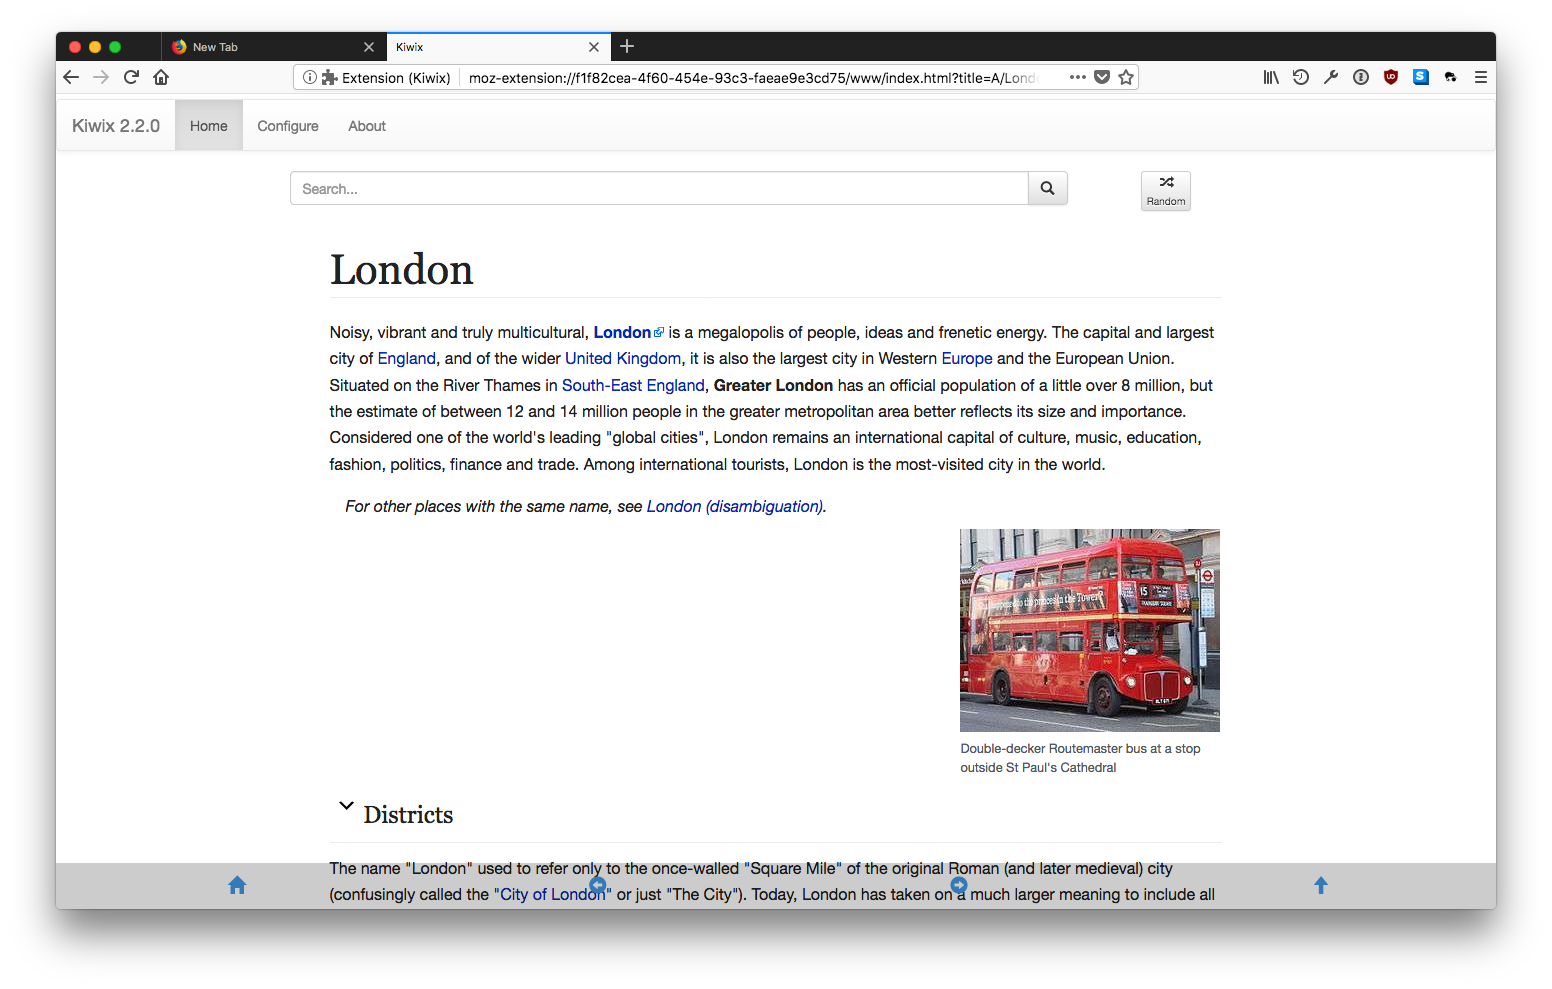
\includegraphics[width=\textwidth]{images/kiwix-js-extension}
		\caption{Kiwix-JS running in FireFox}
		\label{fig:kiwix-firefox}
	\end{center}
\end{figure}

Kiwix JS as it stands has support for Wikimedia and StackOverflow ZIM files (although others may work, just not supported). This meant that if I could get SAFE Wiki working then it would be possible to not only browse Wikimedia content but also content coming from StackOverflow. The content that users could browse on the SAFE Network would be static, but with that comes some benefits.

\section{Static versus Dynamic Content}

When the idea to 'build a Wikipedia on the SAFE Network' first came to mind, I was very well aware of the fact that most likely nobody would use it. It would exist as nothing more than a tech demo with the slight hope that I would be able to continue developing it after I had finished my studies. Getting enough users to start contributing content, and building an environment where strict moderation could occur, would have been a fools-errand. Especially in the time permissible for this project. I just wouldn't have been able to build a full Wiki system on the SAFE Network and do it justice.

It is with that realisation that I came to discover Kiwix. Instead of trying to build a Wiki system on the SAFE Network and trying to bring users across, why not bring Wikipedia (and other sites) to the SAFE Network. This wouldn't be dynamic in anyway (in that users can edit the content) but it would be there for consumption. The storage of the data facilitated by all the features that the SAFE Network has to offer. An important thing about this approach is that by the end of the year I could have a working and browsable copy Wikipedia on the SAFE Network. In its entirety. Not just a simple throwaway tech demo, but a tool that people might actually be able to use.

Websites like Wikipedia only work because of their user base. When a user edits an article this change is logged and anyone can review any changes made. As there are thousands of users anything that is grievously wrong is likely to be flagged and addressed quickly. Similarly if someone is acting as a \textit{bad-party} and editing pages wrongfully (think governments editing pages of staff members to make them appear in a better light) can be blocked based on IP address. This simple measure means that, in most cases, edits are tied to an IP address and hence can be blocked. A simple example is a school, I don't think it needs explaining that school children can be known for being rather silly sometimes. Resulting in the vandalism of some Wikipedia pages. As this is the case it is trivial for Wikipedia to block the IP address(s) that belongs to a school (from making edits) and prevent any further vandalism. On the SAFE Network, this approach is impossible. A user could simply create another account and vandalise an open wiki all they want. It is for reasons such as the ones outlined above that building a dynamic wiki (with adequate moderation techniques/tools) would have been very difficult and most likely a fools errand with the time I have allotted for this project. A static Wiki however, was very achievable.

A static version of Wikipedia might at first seam quite rigid, but in the context of the SAFE Network it makes sense. As the network has a concept of \textit{ownership of data}, a ZIM file that has been uploaded can be directly tied to an account. The ZIM file belongs to someone (an account) in a verifiable \textit{cryptographic} manner. An organisation like Wikimedia, or a trusted third-party, can then upload ZIM files to the network with the assurance that users will know it came from them. It will then exist on the network as an un-censorable mirror (or archive) of whatever source the ZIM file came from. Everyone that has access to the SAFE Network can access it, the only person that is allowed to modify (delete) the file is the holder of the account used to upload the file. As long as you trust the source of the ZIM file, you can \textit{trust} that the information contained within it came from them.

The combination of Kiwix and the SAFE Network makes total sense within this context. A strong pedigree, and the foundation to read and process the ZIM files (static content), meant I could build a tool that could be useful to many people around the world.

\section{Electron}

Electron allows you to "Build cross platform desktop apps with JavaScript, HTML, and CSS". Being able to produce an application that was cross platform was very important to me. The SAFE Network is not platform specific so SAFE Wiki shouldn't be either. As Kiwix JS is built upon web-technologies, Electron seamed like the obvious answer as to how to pull Kiwix JS outside of the web browser environment. Under the hood, Electron combines \textit{Node.js} and \textit{Chromium} into a single environment that can be deployed to the three main platforms: Windows, Linux and macOS. As there exists a \textit{Node.js API} for the SAFE Network this meant that a single application could be built. A single application that could handle both the uploading and deletion of ZIM files on the network and also the browsing of them. The decision not to use the \textit{Web API} to make SAFE Wiki was born out of the requirement of file uploading. To facilitate the upload of large files, (The ZIM for Wikipedia with images is \textgreater 70GB) I really needed to build a desktop application. 

Electron, and indeed Javascript, was very much a new world to me. Beyond simple web development I really haven't done anything note worthy in Javascript. Making Kiwix JS run as an Electron application was hence quite a challenge. After a couple of months of work though I managed to get it running. It was a case of 'completely broken' then one fix lead to 'completely working'. What was now SAFE Wiki, could browse ZIM files from local storage and maintained all the functionality of Kiwix JS.
